%% Journal manuscript for Neural Computing and Applications (Springer).
%% Built on the Springer Nature LaTeX template, Version 3.1 (December 2024).
%% The untouched template, sample article, and user manual are kept in
%% sn-article-template/ for reference.
%%
%% Springer asks for ONE .tex file: do not \input{} or \include{} other
%% .tex files. Keep every file flat in this directory (no subfolders):
%% figures sit next to main.tex and are uploaded as separate files.
%%
%% Build (from this directory):
%%   latexmk -pdf -interaction=nonstopmode -halt-on-error main.tex

%%=====================================================================%%
%% Document class
%%   pdflatex          required by Springer's submission systems
%%   sn-mathphys-num   numbered citations [1]; the class picks the
%%                     matching .bst file, so do NOT add \bibliographystyle
%%   lineno            add for line numbers in the margin (review copies)
%%   referee           add for double line spacing
%% Other reference styles: sn-basic, sn-mathphys-ay, sn-vancouver-num,
%% sn-vancouver-ay, sn-apa, sn-chicago, sn-aps, sn-nature.
%% TODO: confirm NCA's required reference style in its author guidelines.
%%=====================================================================%%
\documentclass[pdflatex,sn-mathphys-num]{sn-jnl}

%%%% Packages (the class already loads hyperref and natbib)
\usepackage{graphicx}%
\usepackage{multirow}%
\usepackage{amsmath,amssymb,amsfonts}%
\usepackage{amsthm}%
\usepackage{mathrsfs}%
\usepackage[title]{appendix}%
\usepackage{xcolor}%
\usepackage{textcomp}%
\usepackage{manyfoot}%
\usepackage{booktabs}%
\usepackage{algorithm}%
\usepackage{algorithmicx}%
\usepackage{algpseudocode}%
\usepackage{listings}%

\theoremstyle{thmstylethree}%
\newtheorem{definition}{Definition}%

\raggedbottom

\begin{document}

%%=====================================================================%%
%% Title and authors
%%=====================================================================%%
%% \title[<short running title>]{<full title>}
\title[Adopt or Retain?]{Adopt or Retain? Testing Sparse Autoencoder Features
as Explanations of Feedback Uptake in a Language Model}

%% Mark the corresponding author with \author* (exactly one).
%% TODO: choose the corresponding author, fill in emails, and confirm
%% author order.
\author[1]{\fnm{Author} \sur{1}}\email{TODO@gwu.edu}
\author[1]{\fnm{Author} \sur{2}}\email{TODO@gwu.edu}
\author[1]{\fnm{Author} \sur{3}}\email{TODO@gwu.edu}
\author[1]{\fnm{Author} \sur{4}}\email{TODO@gwu.edu}
%% TODO: decide whether the advisor is listed as a co-author.
%% \author[1]{\fnm{Amir} \sur{Jafari}}\email{TODO@gwu.edu}

\affil[1]{\orgdiv{Data Science Program}, \orgname{The George Washington
University}, \orgaddress{\city{Washington}, \state{DC}, \country{USA}}}

%%=====================================================================%%
%% Abstract and keywords
%% TODO: check NCA's abstract word limit and keyword count.
%%=====================================================================%%
\abstract{TODO: Abstract 250 - 450 words}


\keywords{sparse autoencoders, mechanistic interpretability, feedback uptake,
activation steering, large language models}

\maketitle

%%=====================================================================%%
%% Main text
%%=====================================================================%%
\section{Introduction}\label{sec:introduction}

TODO JOSH

\section{Related work}\label{sec:related-work}

TODO RAYE

\section{Methods}\label{sec:methods}

\subsection{Solver--Critic pipeline and data}\label{subsec:pipeline-data}

TODO ISRAEL

\subsection{Sparse autoencoders}\label{subsec:saes}

We used sparse autoencoders (SAEs) to represent the Solver's dense activations as sparse latent features \cite{cunningham2023sparse}.
These features provided candidate representations for predicting and intervening on feedback adoption or retention. Sparsity does not,
by itself, establish that a feature represents a single interpretable concept or causally influences the Solver's behavior. We therefore
treated associations between latent features and behavioral outcomes as a screening step, followed by the intervention analysis described in
Section~\ref{subsec:interventions}.

We compared three SAE representations: a custom $L_1$-regularized
SAE trained on interaction activations, a frozen pretrained
Gemma Scope 2 SAE, and a decoder-adapted version of the pretrained
SAE. This comparison evaluated a task-specific dictionary,
an externally pretrained dictionary, and adaptation of the
pretrained reconstruction mapping while preserving its encoder.

\subsubsection{Activation data and preprocessing}

Each SAE input was a $d=2{,}560$-dimensional residual-post activation from Layer 25 of the Solver, collected at the final prompt token immediately
before generation of the second Solver response. Each example therefore contributed one activation vector representing the Solver's state after receiving
the candidate answers and before producing its response.

The Solver used \texttt{google/gemma-3-4b-it} \cite{gemmateam2025gemma3} (revision \texttt{093f9f388b31de276ce2de164bdc2081324b9767}). Layer indices are zero-based, so Layer 25
denotes the output of the 26th transformer block. We selected this layer by comparing Adoption-versus-Retention logistic-regression probes \cite{alain2016probes} across nine 
candidate layers, with regularization tuned using question-family-grouped cross-validation within the training partition. Layer 25 achieved 
the highest validation balanced accuracy and was fixed for subsequent analyses. Test and intervention data were excluded from selection.

Training, validation, test, and intervention partitions followed the question-family grouping described in Section~\ref{subsec:pipeline-data}. Related examples
from the same question family remained in the same partition. Only training activations were used to update SAE parameters. Validation activations
were used for hyperparameter and checkpoint selection; test and intervention activations were excluded from SAE fitting and selection.

For the custom SAEs, inputs were divided by a single scalar root-mean-square value computed from the training activation matrix:
\begin{equation}
s_{\mathrm{RMS}}
=
\sqrt{
\frac{1}{N_{\mathrm{train}}d}
\sum_{i=1}^{N_{\mathrm{train}}}
\sum_{j=1}^{d} x_{ij}^{2}
},
\qquad
\tilde{x}_i = \frac{x_i}{s_{\mathrm{RMS}}}.
\end{equation}

The same frozen scalar was used for all partitions, and reconstructed activations were multiplied by this scalar to restore their original units. The
pretrained SAE and its decoder-adapted variant received raw activations without this normalization.


\subsubsection{Custom sparse autoencoder}

The custom $L_1$ SAE used an encoder with a rectified linear unit
(ReLU) activation and a linear decoder:
\begin{align}
z_i
&=
\operatorname{ReLU}
\left(W_{\mathrm{enc}}\tilde{x}_i+b_{\mathrm{enc}}\right),
\\
\hat{\tilde{x}}_i
&=
W_{\mathrm{dec}}z_i+b_{\mathrm{dec}},
\\
\hat{x}_i
&=
s_{\mathrm{RMS}}\hat{\tilde{x}}_i.
\end{align}
Here, $z_i\in\mathbb{R}^{m}$ is the latent representation,
$m=12{,}888$ is the dictionary width,
$W_{\mathrm{enc}}\in\mathbb{R}^{m\times d}$,
$W_{\mathrm{dec}}\in\mathbb{R}^{d\times m}$,
$b_{\mathrm{enc}}\in\mathbb{R}^{m}$, and
$b_{\mathrm{dec}}\in\mathbb{R}^{d}$.

Training minimized reconstruction error and the mean absolute latent
activation:
\begin{equation}
\mathcal{L}_{L_1}
=
\frac{1}{Nd}
\sum_{i=1}^{N}
\left\|
\tilde{x}_i-\hat{\tilde{x}}_i
\right\|_2^2
+
\lambda
\frac{1}{Nm}
\sum_{i=1}^{N}
\|z_i\|_1,
\end{equation}
where $N$ denotes the number of examples over which the objective
is evaluated and $\lambda$ controls the sparsity penalty. The
encoder was initialized as the transpose of the decoder, after
which their weights were optimized independently. Decoder columns
were normalized to unit $L_2$ norm after each optimizer step,
preventing the model from reducing the latent penalty merely by
increasing decoder magnitudes.


We trained models with $\lambda\in\{1,2,3\}$ and selected $\lambda=2$. Training used Adam \cite{kingma2015adam} with a learning rate $10^{-4}$, shuffled minibatches of 256 examples, seed 42,
and a maximum of 200 epochs. A plateau scheduler reduced the learning rate by a factor of ten with a patience of five. Early stopping used a patience of 20 and an absolute validation-loss 
improvement threshold of $10^{-4}$. The checkpoint with the lowest observed validation objective was retained, including improvements smaller than the early-stopping threshold.

\begin{figure}[htbp]
\centering
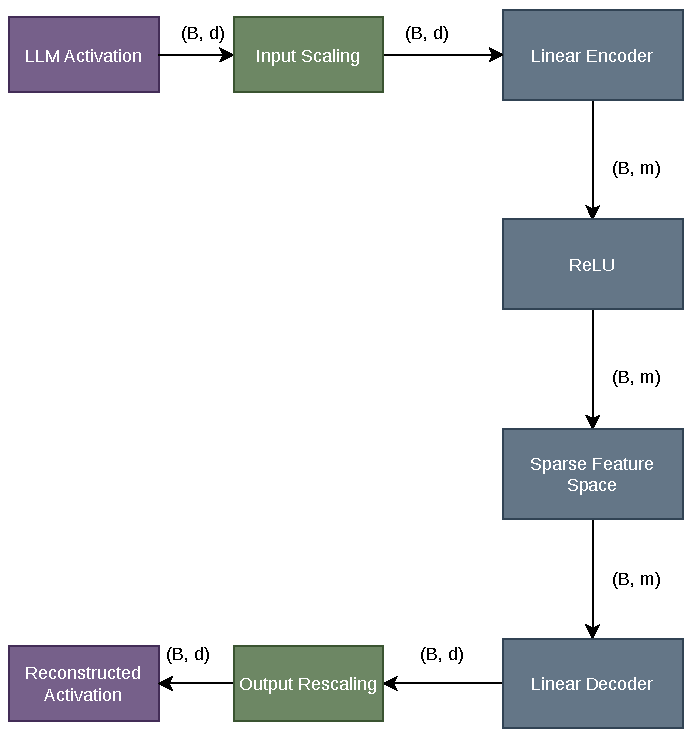
\includegraphics[width=0.6\linewidth]{sae_architecture}
\caption{Custom $L_1$ SAE architecture. An activation vector of
dimension $d=2{,}560$ is divided by the frozen training RMS,
encoded into $m=12{,}888$ nonnegative latent features, and
reconstructed by a linear decoder. The reconstruction is rescaled
to the original activation units}
\label{fig:sae-architecture}
\end{figure}

\subsubsection{Pretrained SAE and decoder-only adaptation}

We used the Gemma Scope 2 SAE from \texttt{google/gemma-scope-2-4b-it}, with identifier \texttt{resid\_post\_all/layer\_25\_width\_16k\_l0\_big}. This SAE maps the same $d=2{,}560$-dimensional 
activation space to $m=16{,}384$ latent features.

The pretrained SAE is part of the Gemma Scope 2 release \cite{mcdougall2025gemmascope2} and uses the JumpReLU architecture \cite{rajamanoharan2024jumping}.

For raw input $x_i$, its encoding and reconstruction are
\begin{align}
a_i
&=
W_{\mathrm{enc}}x_i+b_{\mathrm{enc}},
\\
z_{ij}
&=
\operatorname{ReLU}(a_{ij})
\mathbf{1}\{a_{ij}>\theta_j\},
\\
\hat{x}_i
&=
W_{\mathrm{dec}}z_i+b_{\mathrm{dec}},
\end{align}
where $\theta_j$ is the pretrained threshold for latent feature
$j$ and $\mathbf{1}\{\cdot\}$ denotes the indicator function.
All parameters remained frozen in the unadapted baseline.

To examine adaptation to the interaction activation distribution, we trained a second variant while freezing the encoder weights, encoder bias, and JumpReLU thresholds. Only the decoder weights
and reconstruction bias were updated. Consequently, the frozen and decoder-adapted models produced identical latent activations for identical inputs, while their reconstructions and decoder directions 
could differ. This comparison isolates changes to the reconstruction mapping without relearning the feature detectors.

Latent activations were cached once for the training and validation partitions. Decoder adaptation minimized raw-space reconstruction error:
\begin{equation}
\mathcal{L}_{\mathrm{adapt}}
=
\frac{1}{Nd}
\sum_{i=1}^{N}
\left\|
x_i-\left(W_{\mathrm{dec}}z_i+b_{\mathrm{dec}}\right)
\right\|_2^2.
\end{equation}
We used Adam with a learning rate $10^{-5}$, minibatches of
256 examples, seed 42, a maximum of 10 epochs, and early-stopping
patience of five. The untouched pretrained checkpoint was eligible
for selection as epoch zero. The checkpoint with the lowest
validation reconstruction MSE was retained, and encoder
parameter hashes were checked to verify that the feature
detectors remained unchanged.

Figure~\ref{fig:gemma-scope-sae} summarizes the pretrained
architecture and the parameters updated during adaptation.

\begin{figure}[htbp]
\centering
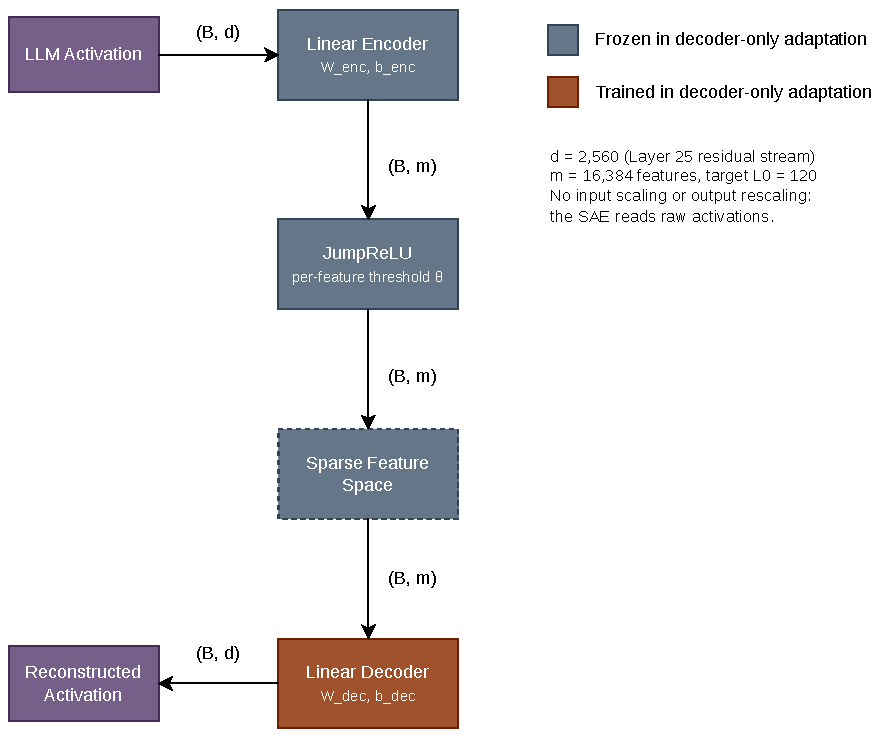
\includegraphics[width=0.75\linewidth]{gemma_scope_sae}
\caption{Pretrained Gemma Scope 2 SAE and decoder-only adaptation.
Raw activations of dimension $d=2{,}560$ are encoded into
$m=16{,}384$ latent features using feature-specific JumpReLU
thresholds. During adaptation, the encoder weights, encoder bias,
and thresholds remain frozen, while the decoder weights and
reconstruction bias are optimized}
\label{fig:gemma-scope-sae}
\end{figure}

\subsubsection{Representation evaluation}


We evaluated reconstruction quality and latent activity separately. Reconstruction MSE was evaluated in RMS-normalized activation units for custom SAEs and in raw activation units for pretrained
and decoder-adapted SAEs:
\begin{align}
\operatorname{MSE}_{\mathrm{custom}}
&=
\frac{1}{Nd}\sum_{i=1}^{N}
\|\tilde{x}_i-\hat{\tilde{x}}_i\|_2^2,
\\
\operatorname{MSE}_{\mathrm{pretrained}}
&=
\frac{1}{Nd}\sum_{i=1}^{N}
\|x_i-\hat{x}_i\|_2^2.
\end{align}
MSE values were therefore not compared directly across the
custom and pretrained model families.
Variance explained was evaluated relative to the training-set
mean activation $\bar{x}_{\mathrm{train}}$:
\begin{equation}
\operatorname{VE}
=
1-
\frac{
\sum_{i=1}^{N}\|x_i-\hat{x}_i\|_2^2
}{
\sum_{i=1}^{N}\|x_i-\bar{x}_{\mathrm{train}}\|_2^2
}.
\end{equation}
We measured sparsity as the mean number of positive latent
features per example:
\begin{equation}
\operatorname{MeanActive}
=
\frac{1}{N}
\sum_{i=1}^{N}
\sum_{j=1}^{m}
\mathbf{1}\{z_{ij}>0\}.
\end{equation}
Feature firing frequency was the fraction of evaluated examples on which a feature was positive. Dictionary coverage was the fraction of features that fired at least once on the evaluated 
partition; features with zero observed firings were classified as inactive on that partition.

Checkpoint selection was completed before test evaluation. Reconstruction quality and sparsity were treated as representation diagnostics, not as evidence of semantic interpretability or 
causal influence. Because the custom and pretrained SAEs differed in dictionary width, sparsity mechanism, and training distribution, their comparison evaluates the resulting representations rather
than isolating the effect of any single architectural choice.

\subsection{Prediction probes}\label{subsec:probes}

TODO RAYE

\subsection{Causal interventions}\label{subsec:interventions}

TODO RAYE

\section{Results}\label{sec:results}

TODO ISRAEL

\section{Discussion}\label{sec:discussion}

TODO JOSH

\section{Conclusion}\label{sec:conclusion}

TODO JOSH

%%=====================================================================%%
%% Back matter
%%=====================================================================%%
\backmatter

\bmhead{Acknowledgements}

TODO ISRAEL

%% Springer requires every heading below. Write "Not applicable" for any
%% heading that does not apply; do not delete headings.
\section*{Declarations}

\begin{itemize}
\item \textbf{Funding:} TODO.
\item \textbf{Competing interests:} TODO.
\item \textbf{Ethics approval and consent to participate:} TODO.
\item \textbf{Consent for publication:} TODO.
\item \textbf{Data availability:} TODO.
\item \textbf{Materials availability:} TODO.
\item \textbf{Code availability:} TODO.
\item \textbf{Author contribution:} TODO.
\end{itemize}

%%=====================================================================%%
%% Appendices (delete the environment if none are needed)
%%=====================================================================%%
\begin{appendices}

\section{TODO appendix title}\label{secA1}

TODO ISRAEL


\begin{algorithm}[H]
\caption{Custom L1 or TopK--AuxK SAE training}
\label{alg:custom-sae-training}
\begin{algorithmic}[1]
\Require Training activations $X_{\mathrm{train}}$; validation activations $X_{\mathrm{val}}$;
sparsity mode $q\in\{L_1,\mathrm{TopK}\}$; dictionary width $m$; maximum epochs $E$;
batch size $B$; learning rate $\eta$
\Ensure Frozen SAE checkpoint with the lowest main-path validation loss
\State $s_{\mathrm{RMS}}\gets\sqrt{\operatorname{mean}(X_{\mathrm{train}}^2)}$
\State Initialize tied encoder--decoder weights and normalize every decoder column
\State Initialize Adam, the plateau scheduler, inactivity counters, and early stopping
\For{$e=1$ to $E$}
    \For{each shuffled minibatch $X\subset X_{\mathrm{train}}$ of size $B$}
        \State $\widetilde{X}\gets X/s_{\mathrm{RMS}}$
        \State $A\gets W_{\mathrm{enc}}\widetilde{X}+b_{\mathrm{enc}}$
        \If{$q=L_1$}
            \State $Z\gets\operatorname{ReLU}(A)$
            \State $\mathcal{L}\gets\mathcal{L}_{\mathrm{rec}}+\lambda\operatorname{mean}(|Z|)$
        \Else
            \State $P\gets\operatorname{ReLU}(A)$; $Z\gets\operatorname{TopK}(P,k)$
            \State Update each feature's last main-path firing position from $Z$
            \State $J\gets$ features inactive for at least $w$ training examples
            \If{$J\ne\emptyset$ and the inactivity warm-up is complete}
                \State $Z_{\mathrm{aux}}\gets
                \operatorname{TopK}(P|_J,\min(k_{\mathrm{aux}},|J|))$
                \State $R\gets(\widetilde{X}-\widehat{\widetilde{X}})\text{.detach}()$
                \State $\mathcal{L}\gets\mathcal{L}_{\mathrm{rec}}+
                \alpha\operatorname{MSE}(W_{\mathrm{dec}}Z_{\mathrm{aux}},R)$
            \Else
                \State $\mathcal{L}\gets\mathcal{L}_{\mathrm{rec}}$
            \EndIf
        \EndIf
        \State Update SAE parameters with Adam using $\nabla\mathcal{L}$
        \State Renormalize every decoder column to unit $L_2$ norm
    \EndFor
    \State Evaluate the main-path objective on $X_{\mathrm{val}}$ without AuxK
    \State Update the scheduler and save any new lowest-loss checkpoint
    \If{validation loss has no significant improvement for the patience window}
        \State \textbf{break}
    \EndIf
\EndFor
\State Reload and freeze the lowest-loss checkpoint
\State \Return frozen SAE and split-level reconstruction and activity metrics
\end{algorithmic}
\end{algorithm}


\begin{algorithm}[H]
\caption{Decoder-only adaptation of the pretrained SAE}
\label{alg:decoder-only-adaptation}
\begin{algorithmic}[1]
\Require Pretrained JumpReLU SAE $f$; training activations $X_{\mathrm{train}}$;
validation activations $X_{\mathrm{val}}$; epochs $E$; batch size $B$; learning rate $\eta$
\Ensure Adapted decoder with unchanged encoder features and thresholds
\State Load $f$ and digest $(W_{\mathrm{enc}},b_{\mathrm{enc}},\theta)$
\State Freeze $W_{\mathrm{enc}}$, $b_{\mathrm{enc}}$, and JumpReLU thresholds $\theta$
\For{$S\in\{X_{\mathrm{train}},X_{\mathrm{val}}\}$}
    \State Cache $Z_S\gets\operatorname{JumpReLU}(W_{\mathrm{enc}}S+b_{\mathrm{enc}};\theta)$ once
\EndFor
\State Evaluate the untouched SAE and bias-only recentered baseline
\State Initialize Adam over only $(W_{\mathrm{dec}},b_{\mathrm{dec}})$
\State Save the untouched model as eligible epoch 0
\For{$e=1$ to $E$}
    \For{each shuffled minibatch $(Z,X)$ from the cached training codes}
        \State $\widehat{X}\gets W_{\mathrm{dec}}Z+b_{\mathrm{dec}}$
        \State $\mathcal{L}\gets\operatorname{MSE}(\widehat{X},X)$
        \State Update only $(W_{\mathrm{dec}},b_{\mathrm{dec}})$ with Adam
    \EndFor
    \State Evaluate validation reconstruction using the cached validation codes
    \If{validation MSE is lower than the best eligible MSE}
        \State Save the decoder and reconstruction bias; reset patience
    \Else
        \State Increment the early-stopping counter
    \EndIf
    \If{the counter reaches the patience limit}
        \State \textbf{break}
    \EndIf
\EndFor
\State Reload the best checkpoint and verify the encoder digest is unchanged
\State \Return adapted SAE, provenance manifest, and before--after metrics
\end{algorithmic}
\end{algorithm}

\end{appendices}

%%=====================================================================%%
%% References: entries live in references.bib
%%=====================================================================%%
\bibliography{references}

\end{document}
